\chapter{D-algorithm}
\label{sec:p2-d-algorithm}
% P2: bản ngắn; bảng đầy đủ và trace chi tiết nằm trong tests/data và notes.
\textbf{D-calculus và các cube.}
D-algorithm của Roth (1966) biểu diễn sai khác giữa mạch tốt và mạch lỗi
bằng $D=(1,0)$, $D'=(0,1)$; $0=(0,0)$, $1=(1,1)$ và $X$ chưa biết
\cite{p2_roth1966}. Đánh giá cổng riêng trên hai thành phần rồi ghép kết quả:
$D\land1=D$, $D\land D'=0$, $D\land X=X$,
$\operatorname{NAND}(D,1)=D'$. Nhóm lập bảng đầy đủ cho tám loại cổng và
dùng làm dữ liệu kiểm thử chung cho chương trình.
Với NAND $z=\overline{ab}$, singular cover gồm $(0,X,1)$, $(X,0,1)$,
$(1,1,0)$. PDCF cho $z/\mathrm{SA0}$ là $(0,X,D)$ hoặc $(X,0,D)$;
PDC như $(D,1,D')$ đưa sai khác qua cổng. D-intersection kết hợp
các yêu cầu cùng net: $X\cap v=v$, $v\cap v=v$; hai giá trị xác định khác
nhau gây xung đột khi cực $D/D'$ đã cố định.

\textbf{Tìm kiếm và justification.}
D-frontier chứa cổng có đầu vào $D/D'$ nhưng đầu ra $X$;
J-frontier chứa cổng có đầu ra đã gán nhưng đầu vào chưa justify được.
Thuật toán chọn PDCF, thực hiện implication tiến/lùi, chọn PDC để đưa lỗi
ra PO, rồi dùng singular cover justify các yêu cầu nội bộ. Khi xung đột,
khôi phục trạng thái và thử cube khác. Chỉ thành công khi sai khác tới PO
\emph{và} mọi yêu cầu đều nhất quán, được thực hiện bởi PI. Lưu đồ ở
Hình~\ref{fig:p2-flow}.
\begin{figure}[htbp]
\centering
% Chỉ dùng các thư viện TikZ đã có trong main.tex của P1.
\begin{tikzpicture}[>=Stealth,
  every node/.style={font=\scriptsize,align=center},
  p2box/.style={draw,rounded corners,minimum height=7mm,text width=2.5cm}]
\node[p2box] (fault) at (0,0) {Chọn PDCF\\kích hoạt lỗi};
\node[p2box] (imply) at (3.1,0) {Implication\\giao cube, kiểm tra};
\node[p2box] (drive) at (6.2,0) {Chọn PDC\\lan truyền tới PO};
\node[p2box] (justify) at (9.3,0) {Singular cover\\justify tới PI};
\node[p2box] (back) at (3.1,-1.15) {Xung đột: khôi phục\\thử cube khác};
\node[p2box] (done) at (9.3,-1.15) {PO có D/D'; J rỗng\\thành công};
\draw[->] (fault)--(imply);
\draw[->] (imply)--(drive);
\draw[->] (drive)--(justify);
\draw[->] (justify)--(done);
\draw[->] (imply)--(back);
\draw[->] (back.west) to[bend left=35] node[left]{thử lại} (imply.west);
\draw[->] (drive.north) to[bend right=25] node[above]{imply lại} (imply.north);
\draw[->] (justify.south west)--(back.north east);
\end{tikzpicture}

\caption{Luồng D-algorithm; khôi phục cả gán net và frontier khi quay lui.}
\label{fig:p2-flow}
\end{figure}

\textbf{Ví dụ c17, lỗi stem $11/\mathrm{SA0}$.}\par
Bảng~\ref{tab:p2-trace} ghi bốn lần chọn cube; không đếm các lần implication.
Ở bước 3, $22=D$ chưa đủ kết luận thành công vì net 10 còn cần justification.
\begin{table}[htbp]
\centering\small
\caption{Chạy tay D-algorithm: $J$ ghi các net đầu ra chưa justify.}
\label{tab:p2-trace}
\begin{tabular}{@{}clll@{}}
\toprule
Bước & Cube trên các net & Implication chính & $J$\\
\midrule
1 & PDCF $(3,6,11)=(X,0,D)$ & $11=D$ & $\varnothing$\\
2 & PDC $(2,11,16)=(1,D,D')$ & $16=D'$ & $\varnothing$\\
3 & PDC $(10,16,22)=(1,D',D)$ & $22=D$ & $\{10\}$\\
4 & Cover $(1,3,10)=(X,0,1)$ & Gán PI $3=0$ & $\varnothing$\\
\bottomrule
\end{tabular}
\end{table}
Theo thứ tự PI $(1,2,3,6,7)$, thu được $(X,1,0,0,X)$, điền $X=0$ thành
$01000$. Bốn cách điền đều cho $22_{\rm tốt}=1$, $22_{\rm lỗi}=0$.
Sau kiểm chứng có thể bỏ ràng buộc $6=0$, được $(X,1,0,X,X)$;
đây là bước tổng quát hóa cube, không phải một quyết định tìm kiếm.
Ví dụ có \textbf{4 lần chọn cube, 0 backtrack}; không dùng nó để kết luận
D-algorithm luôn ít bước hơn PODEM.\par
\begin{figure}[htbp]
\centering
% P2: tái sử dụng hình mach_c17.jpg do người dùng cung cấp, không vẽ lại.
% Wrapper dùng được từ report/main.tex và slides/main.tex.
% Hình thể hiện cube tổng quát hóa (X,1,0,X,X).
\IfFileExists{figures/common/mach_c17.jpg}{%
  \includegraphics[width=0.72\linewidth]{figures/common/mach_c17.jpg}%
}{%
  \includegraphics[width=0.72\linewidth]{../report/figures/common/mach_c17.jpg}%
}

\caption{Mạch c17 với cube sau tổng quát hóa, $6=X$;
đường quan sát $11=D\to16=D'\to22=D$.}
\label{fig:p2-c17}
\end{figure}

\textbf{Nhận xét.}
Quyết định trên net nội bộ tạo thêm công việc justification; fanout hội tụ
có thể làm các yêu cầu cục bộ xung đột hoặc che sai khác. Trong c17, ảnh
hưởng net 11 đi qua 16 và 19 rồi hội tụ tại 23. Tìm kiếm có thể tăng theo
cấp số mũ trong trường hợp xấu; PODEM hạn chế quyết định tại PI
(Chương~\ref{sec:p3-podem}). Sách Bushnell--Agrawal là tài liệu đọc bổ sung
\cite{p2_bushnell2000}; ví dụ và số bước trên đây là chạy tay, không phải
kết quả đo từ chương trình.
